\section{Fouriertransformation}

Die Fouriertransformation führt eine Funktion vom Zeitbereich in den Frequenzbereich über. Die Rücktransfomration 
(inverse Fouriertransformation) macht dies wieder rückgängig.

\begin{center}
    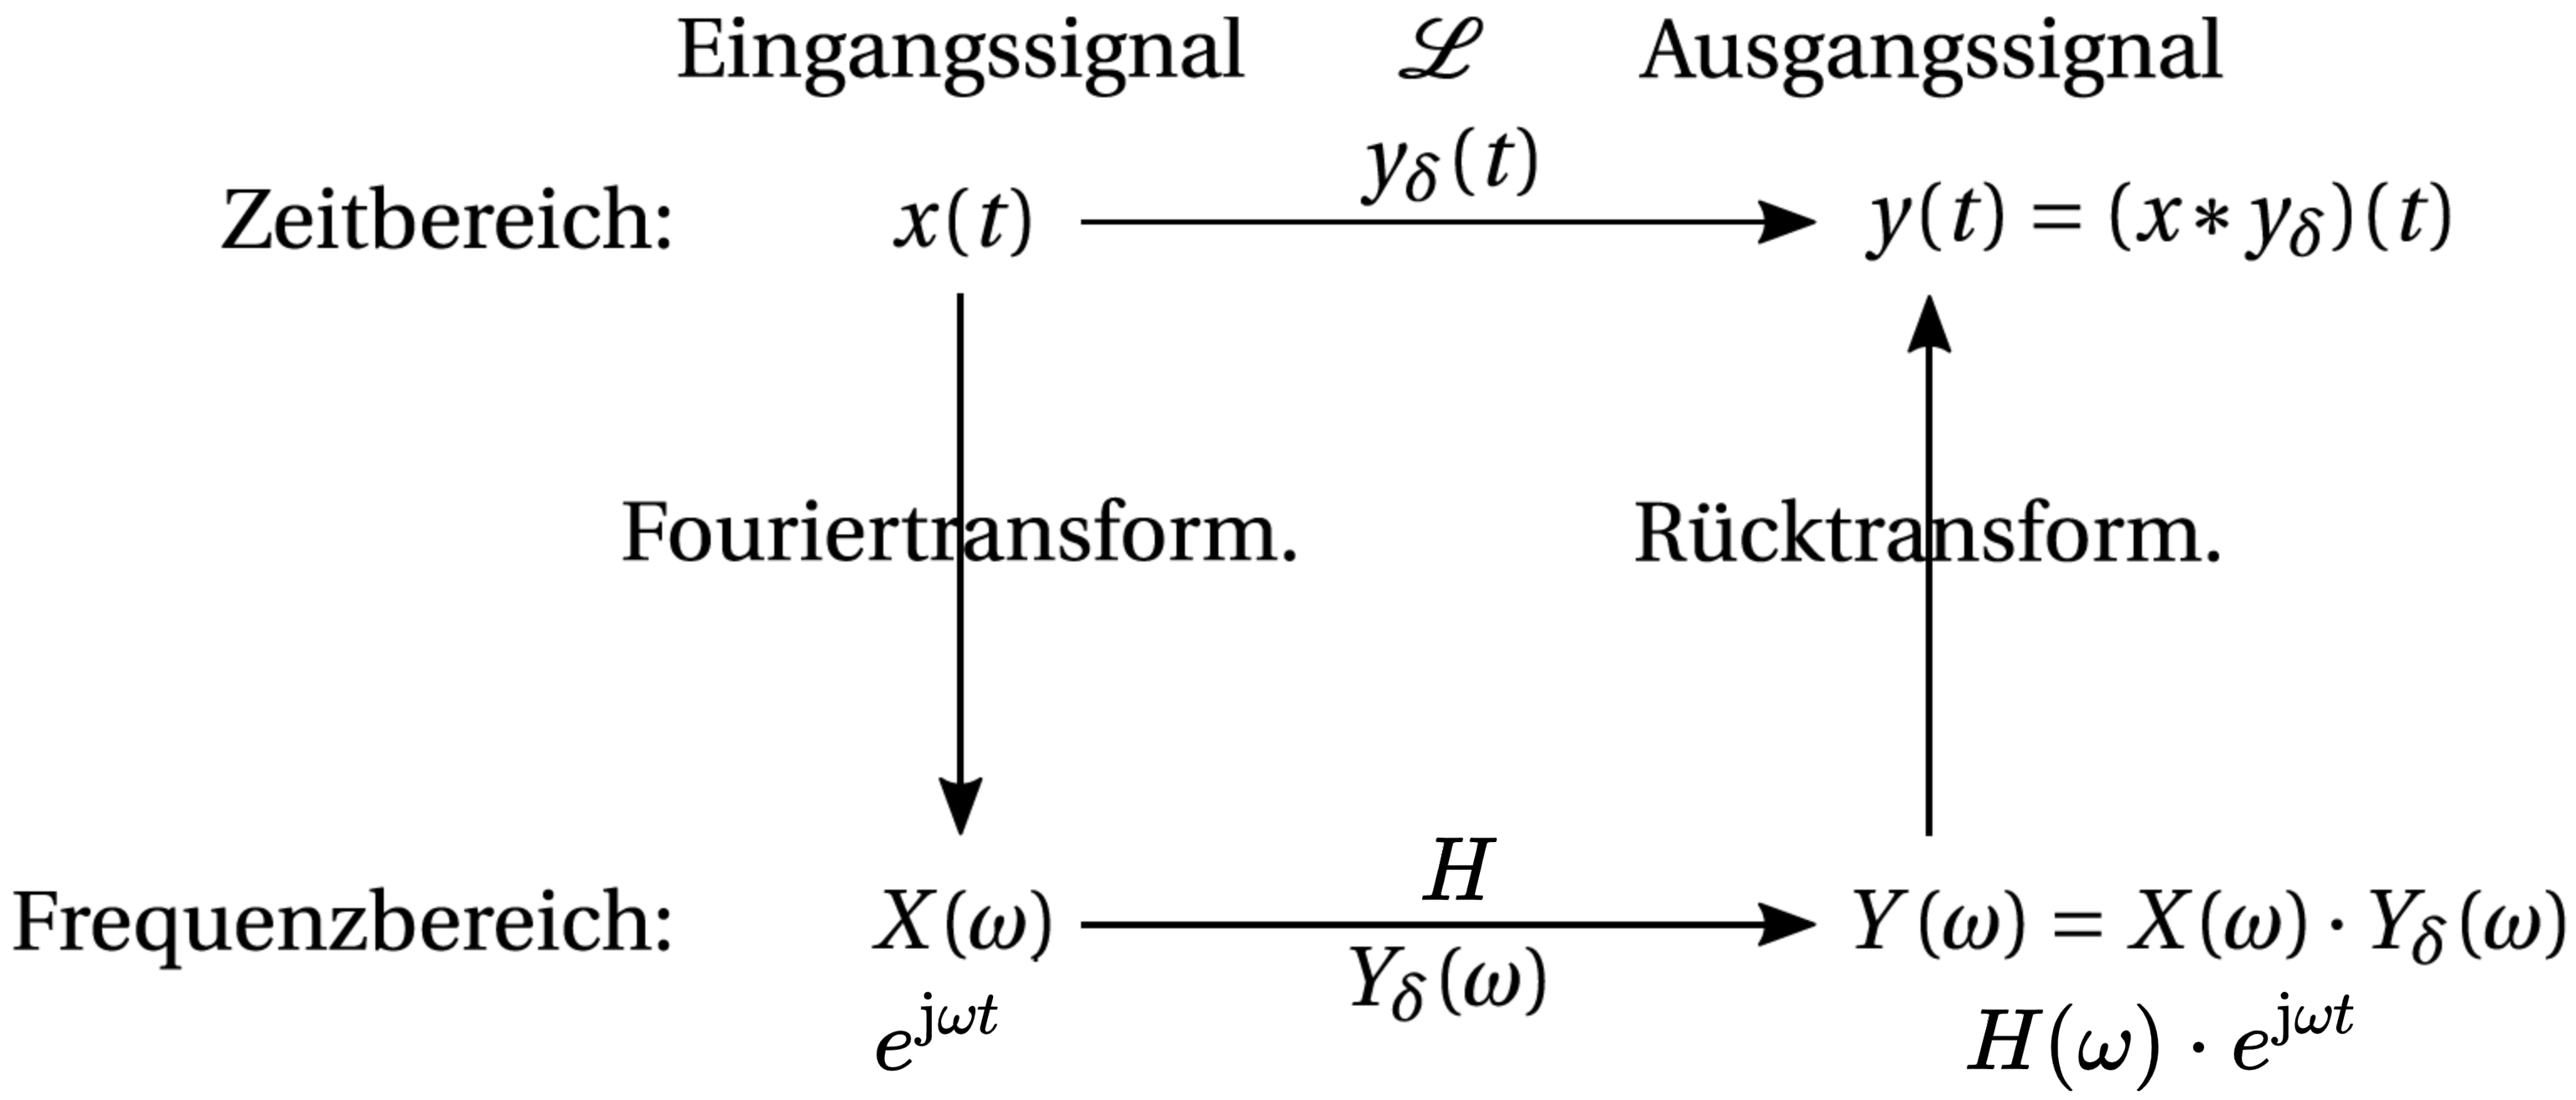
\includegraphics[width=0.7\columnwidth]{images/zeitbereich_frequenzbereich.png}
\end{center}

\vspace{-0.2cm}


\subsection{Komplexe trigonometrische Funktionen} 

\begin{tabular}{lll}
    $\sin(\omega t) = \frac{\e^{\jimg\omega t} - \e^{-\jimg \omega t}}{2\jimg}$ &
    $\cos(\omega t) = \frac{\e^{\jimg \omega t} + \e^{-\jimg \omega t}}{2}$ & 
    $\tan(\omega t) = \frac{\sin(\omega t)}{\cos(\omega t)}$
\end{tabular}


\subsection{Frequenzgang (Frequenzerhaltung)}

Der Frequenzgang $H(\omega)$ bestimmt die Änderung von Amplitude und Phase des Eingangssignals.

\textbf{Amplitudengang:} $ A(\omega) = \left|H(\omega)\right| = \sqrt{H(\omega) \cdot \overline{H(\omega)}} = \sqrt{\Re(H(\omega))^2 + \Im(H(\omega))^2}$

\vspace{0.2cm}

\textbf{Phasengang:} $\Phi(\omega) = \arg(H(\omega)) = \begin{cases}
\arccos\left(\frac{ \Re(H(\omega))}{|H(\omega)|}\right)  & \text{für} \; \Im(H(\omega)) \geq 0 \\
-\arccos\left(\frac{ \Re(H(\omega))}{|H(\omega)|}\right) & \text{für} \; \Im(H(\omega)) < 0
\end{cases}$

\vspace{0.2cm}

\begin{tabular}{ll}
    Amplitudengang: & achsensymmetrisch (gerade)    \\
    Phasengang:     & punktsymmetrisch (ungerade)
\end{tabular}


\subsection{Systemantwort berechnen}

Die Systemantwort $y(t)$ (Ausgangssignal) auf ein \cbl{Eingangssignal $x(t)$} berechnet sich mit dem Frequenzgang $H(\omega)$ 
$$ y(t) = H(\omega) \cdot \cbl{x(t)} \qquad \qquad \mathcal{L} \{ \cbl{ \e^{\jimg \omega  t} } \} = H(\omega) \cdot \e^{\jimg \omega t} $$ 


\example{Systemantwort $y(t)$ berechnen}

\vspace{-0.2cm}
$$\cbl{x(t) = \sin(2t)} \qquad H(2) = \frac{-3-2\jimg}{13} \qquad H(-2) = \frac{-3+2\jimg}{13}$$
\vspace{-0.4cm}

\begin{align*}
    y(t)    &= \mathcal{L} \Big\{ \frac{1}{2 \jimg}  \left( \e^{\jimg 2t} - \e^{- \jimg 2t} \right) \Big\} = \frac{1}{2 \jimg} \left(H(2) \cdot \e^{\jimg 2t} - H(-2) \cdot \e^{-\jimg 2t} \right) \\
            &= \frac{1}{2\jimg} \left( \frac{-3-2\jimg}{13} \cdot \e^{\jimg2t} - \frac{-3+2\jimg}{13} \cdot \e^{-\jimg2t} \right) \\
            &= -\frac{3}{13} \underbrace{ \frac{1}{2\jimg} \left( \e^{\jimg2t} - \e^{-\jimg2t} \right)}_{\substack{\sin(2t)}} + \frac{-2 \jimg}{13}  \frac{1}{ \jimg} \underbrace{ \frac{1}{2} \left( \e^{\jimg2t} + \e^{-\jimg2t} \right)}_{\substack{\cos(2t)}}
\end{align*}

\begin{itemize}
    \item Realteil und Imaginärteil \textbf{getrennt} ausklammern! \\
        \textbf{Hinweis:} Wenn $x(t)$ und $y(t)$ bekannt sind, $H(\omega)$ allerdings nur mit Parametern gegeben ist, dann wird mit Ansatz
        $y(t) = H(\omega) \cdot x(t)$ mit Parametern gerechnet
    \item Mit Koeffizientenvergleich fehlende Parameter bestimmen
\end{itemize}


\subsection{Berechnung der Fouriertransformation}

Wenn eine Funktion $f(t)$ im Zeitbereich absolut integrierbar ist, d.h. $\int \limits_{-\infty}^{\infty} | f(t) | \,  \diff t < \infty$, 
dann funktioniert die Umwandlung:

\renewcommand{\arraystretch}{2.5}
\begin{tabular}{ll}
    Fouriertransformierte:  & $F(\omega) = \int \limits_{-\infty}^{\infty} f(t) \, \e^{- \jimg \omega t} \, \diff t$                    \\
    Rücktransformation:     & $f(t) = \frac{1}{2 \pi} \int \limits_{-\infty}^{\infty} F(\omega) \, \e^{\jimg \omega t} \, \diff \omega$
\end{tabular}
\renewcommand{\arraystretch}{1}


\subsubsection{Darstellung der Fouriertransformierten}

\begin{tabular}{ll}
    Spektraldichte:     & entspricht der Fouriertransformierten $F(\omega)$     \\
                        & Die komplexwertige Funktion wird für die Darstellung  \\ 		    
                        & aufgeteilt in Folgendes: \\
    \\
    Amplitudendichte:   & $\vert F(\omega) \vert$ \quad (Betrag der Fouriertransformierten)     \\
    Phasendichte:       &  $\mathrm{arg}( F(\omega))$ \quad (Winkel der Fouriertransformierten)
\end{tabular}


\subsection{Eigenschaften / Rechenregeln Fouriertransformation}

\textbf{\textrightarrow\ siehe Tabelle!}

\textbf{Es folgen Ergänzungen zur Tabelle}	


\subsubsection{Sprungstellen / Symmetrie}

\begin{itemize}
    \item An allfälligen \textbf{Sprungstellen} von $f(t)$ konvergiert die Rücktransformierte von $F(\omega)$ gegen die 
        \textbf{Mitte} der Sprungstelle
    \item Ist $f(t)$ \textbf{gerade}, so hat $F(\omega)$ nur \textbf{reelle} Funktionwerte
    \item Ist $f(t)$ \textbf{ungerade}, so hat $F(\omega)$ nur \textbf{imaginäre} Funktionwerte
\end{itemize}


\subsubsection{Vertauschungssatz; Zeit-Frequenz-Symmetrie}

Ist $f(t) \; \laplace \; F(\omega)$ ein Korrespondenzpaar, dann ist auch $F(t) \; \laplace \; 2 \pi f(-\omega)$ ein Korrespondenzpaar.


\subsubsection{Satz von Parseval / Plancherel}
Ist $F(\omega)$ die Fouriertransformierte von $f(t)$, so gilt

$\int \limits_{-\infty}^{\infty} \vert f(t) \vert ^2 \, \diff t
= \frac{1}{2 \pi} \int \limits_{-\infty}^{\infty} \vert F(\omega) \vert ^2 \, \diff \omega $
, falls $\int \limits_{-\infty}^{\infty} \vert f(t) \vert ^2 \, \diff t$ existiert


\subsection{Wichtige Korrespondenzpaare}

\renewcommand{\arraystretch}{1.5}
\begin{tabular}{r c l}
    $\cos(\omega_0 \, t)$   & $\laplace$    & $\pi(\delta( \omega + \omega_0) + \delta ( \omega - \omega_0))$       \\
    $\sin(\omega_0 \, t)$   & $\laplace$    & $\jimg \pi(\delta( \omega + \omega_0) - \delta ( \omega - \omega_0))$
\end{tabular}
\renewcommand{\arraystretch}{1}


\subsection{Fouriertransformierte einer Fourierreihe}

\vspace{-0.2cm}
$$ f(t) = \sum \limits_{k = - \infty}^{\infty} c_k \, \e^{\jimg k \omega_0 t} \;  \laplace \; 
F(\omega) = 2 \pi \sum \limits_{k = - \infty}^{\infty} c_k \, \delta(\omega - k \omega_0) $$


\subsection{Sampling zeitlich kontinuierlicher Signale}

Mathematisch wird das abzutastende Signal $x(t)$ mit einem \textbf{Dirac-Kamm $\bm{\delta_T(t)}$} multipliziert.
$$ \text{Dirac-Kamm:} \quad \delta_T(t) = \sum \limits_{n = - \infty}^{\infty} \delta(t - nT)$$

Es resultiert das abgetastete Signal $x_a (t)$
$$ x_a (t) = \sum \limits_{n = - \infty}^{\infty} x(t) \cdot \delta(t - nT) = \sum \limits_{n = - \infty}^{\infty} \underbrace{x(nT)}_{\substack{x[n]}} \cdot \delta(t - nT) $$

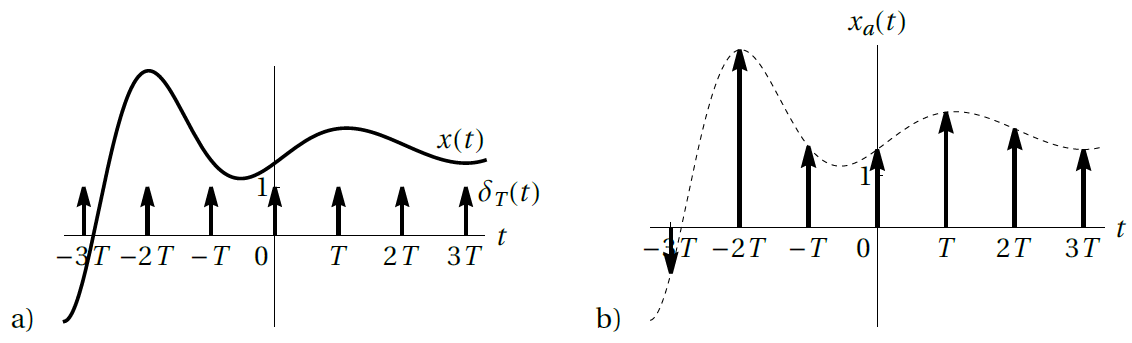
\includegraphics[width=\columnwidth]{images/sampling.png}

\vspace{0.2cm}

\textbf{Wechsel in den Frequenzbereich (Fouriertransformierte)}
$$ x_a (t) = \sum \limits_{n = - \infty}^{\infty} x[n]\cdot \delta(t - nT)  \; \laplace \; 
X_a(\omega) = \frac{1}{T} \sum \limits_{n = - \infty}^{\infty} X(\omega - n \omega_a) \quad \text{mit } \omega_a = \frac{2 \pi}{T} $$		 


\subsection{Diskrete Fouriertransformation (DFT)}

$x[n]$ ist für $n \in \{ 0, \, ... \, , N-1 \} $ eine endliche Folge von reellen Zahlen

\vspace{0.2cm}

\renewcommand{\arraystretch}{2.8}
\begin{tabular}{ll}
    $x[n] = \sum \limits_{k = 0}^{N-1} c_k \, e^{\jimg k (2 \pi / N) \, n}$                 & für $n \in \{ 0, \, \ldots \, , N-1 \}$ \\
    $c_k = \frac{1}{N} \sum \limits_{n = 0}^{N-1} x[n] \, e^{- \jimg k (2 \pi / N) \, n}  $ & für $k \in \{ 0, \, \ldots \, , N-1 \}$ 
\end{tabular}				
\renewcommand{\arraystretch}{1}


\example{Abtastwerte $x[n]$ finden}

\begin{minipage}[c]{0.55\columnwidth}
    Ein Signal $s(t)$ wird auf dem Intervall [0,1] mit der Frequenz $f_a = 4 \, \text{Hz}$ abgetastet.
\end{minipage}
\hfill
\begin{minipage}[c]{0.38\columnwidth}
    $s(t) = \begin{cases}			
        t(1-t)  & \text{für} \; t \in [0,1] \\
        0       & \text{sonst} 
    \end{cases}$  
\end{minipage}

\vspace{0.2cm}

\renewcommand{\arraystretch}{2}
\begin{tabular}{lll}
    $x[0] = s(0) = 0$                                                                               & & 
    $x[1] = s\left( \frac{1}{4} \right) = \frac{1}{4} \left( 1 - \frac{1}{4} \right) = \frac{3}{16}$    \\
    $x[2] = s \left( \frac{1}{2} \right) = \frac{1}{2} \left(1- \frac{1}{2} \right) = \frac{1}{4}$  & &
    $x[3] = s \left( \frac{3}{4} \right) = \frac{3}{4} \left (1 - \frac{3}{4} \right) = \frac{3}{16}$
\end{tabular}
\renewcommand{\arraystretch}{1}


\subsection{Schnelle Fouriertransformation (FFT)}

\textbf{Bedingung:} Die Länge $N$ der endlichen Folge $x[0], \, \ldots \, , x[N-1]$ muss einer Zweierpotenz entsprechen! 
\textrightarrow\ $N = 2^p \; \text{ mit } \; p \in \mathbb{N}$


\subsubsection{Fourierkoeffizienten $c_k$ für $k < \frac{N}{2}$}

\vspace{-0.2cm}

\renewcommand{\arraystretch}{2.5}
\begin{tabular}{ll}
    $c_k = \frac{1}{N} \left( c_{g,k} + E_N^k \, c_{u,k} \right)$   & mit $E_N := e^{-\jimg(2 \pi/N)}$  \\
    $c_{g,k}:= \sum \limits_{m = 0}^{N/2-1} x[2m] \,  E_N^{k2m}$    & $c_{u,k}:= \sum \limits_{m = 0}^{N/2-1} x[2m+1] \,  E_N^{k2m}$
\end{tabular}


\subsubsection{Fourierkoeffizienten $c_{k + N/2}$ }

\vspace{-0.2cm}
\begin{tabular}{l}
    $c_{k + N/2} =  \frac{1}{N} \left( c_{g,k} - E_N^k \, c_{u,k} \right)$
\end{tabular}
\renewcommand{\arraystretch}{1}

\columnbreak

